\documentclass[11pt,letterpaper,twoside]{book}

% ==========================================
% SIRC-1 CPU Reference Manual
% SIR Compute Using Load/store ALU and Registers
% ==========================================

% ==========================================
% Preamble for SIRC-1 CPU Reference Manual
% ==========================================

% ------------------------------------------------------------
% Encoding and typography
% ------------------------------------------------------------

\usepackage[utf8]{inputenc}
\usepackage[T1]{fontenc}

% Helvetica-compatible sans serif.
% TeX Gyre Heros is a high-quality Helvetica replacement.
\usepackage{tgheros}
\renewcommand{\familydefault}{\sfdefault}

% Courier-compatible monospace.
\usepackage{tgcursor}

% Better character spacing / kerning.
\usepackage{microtype}


% ------------------------------------------------------------
% Page layout
% ------------------------------------------------------------

\usepackage{geometry}

\geometry{
    a4paper,
    left=25mm,
    right=20mm,
    top=22mm,
    bottom=25mm,
    headheight=14pt
}


% ------------------------------------------------------------
% General packages
% ------------------------------------------------------------

\usepackage{graphicx}
\usepackage{xcolor}
\usepackage{fancyhdr}
\usepackage{titlesec}
\usepackage{enumitem}
\usepackage{float}

\usepackage{tabularx}
\usepackage{booktabs}
\usepackage{multirow}
\usepackage{longtable}
\usepackage{xltabular}

\usepackage{amsmath}
\usepackage{amssymb}

\usepackage{listings}
\usepackage{bytefield}

\usepackage{tikz}
\usepackage{tikz-timing}
\usetikzlibrary{
    shapes.geometric,
    arrows.meta,
    positioning,
    fit,
    calc
}

\usepackage{tcolorbox}
\tcbuselibrary{breakable, skins}

% Load hyperref relatively late.
\usepackage{hyperref}


% ------------------------------------------------------------
% Timing diagrams
% ------------------------------------------------------------

\tikzset{
    sirc timing diagram/.style={
        timing/slope=0,
        timing/dslope=0.15,
        timing/xunit=3.4em,
        timing/rowdist=2.2,
        timing/coldist=2.2,
    },
}


% ------------------------------------------------------------
% Colours
% ------------------------------------------------------------

\definecolor{sircred}{RGB}{255,0,0}
\definecolor{sircgray}{RGB}{110,110,110}
\definecolor{sirclightgray}{RGB}{232,232,232}
\definecolor{codebg}{RGB}{245,245,245}
\definecolor{opcodecolor}{RGB}{153,0,0}


% ------------------------------------------------------------
% Header / footer
% ------------------------------------------------------------

\pagestyle{fancy}
\fancyhf{}

\fancyhead[LE]{\small\nouppercase{\leftmark}}
\fancyhead[RO]{\small\nouppercase{\rightmark}}

\fancyfoot[LE,RO]{\thepage}
\fancyfoot[C]{\small\textcolor{sircgray}{SIRC-1 REFERENCE MANUAL}}

\renewcommand{\headrulewidth}{0.8pt}
\renewcommand{\footrulewidth}{0.4pt}


% ------------------------------------------------------------
% PDF / hyperlink setup
% ------------------------------------------------------------

\hypersetup{
    colorlinks=true,
    linkcolor=sircred,
    filecolor=sircred,
    urlcolor=sircred,
    citecolor=sircred,
    bookmarksnumbered=true,
    pdfauthor={SIRC Development Team},
    pdftitle={SIRC-1 CPU Reference Manual},
    pdfsubject={SIRCIS Instruction Set Architecture},
}


% ------------------------------------------------------------
% Assembly code listings
% ------------------------------------------------------------

\lstdefinelanguage{SIRC}{
    morekeywords={
        ADDI,ADDR,ADCI,ADCR,SUBI,SUBR,SBCI,SBCR,
        ANDI,ANDR,ORRI,ORRR,XORI,XORR,
        LOAD,STOR,CMPI,CMPR,TSAI,TSAR,TSXI,TSXR,
        LDEA,LDEL,BRAN,LJMP,LJSR,BRSR,RETS,NOOP,
        WAIT,RETE,COPI,COPR,SHFT,EXCP,RSET,
        ETFR,ETTR,DMAR,DMAW,DMAT,MULU,MULS,DIVU,DIVS
    },
    keywordstyle=\color{sircred}\bfseries,
    sensitive=false,
    morecomment=[l]{;},
    commentstyle=\itshape\color{sircgray},
    morestring=[b]",
    stringstyle=\color{opcodecolor},
    basicstyle=\ttfamily\small,
    breaklines=true,
    showstringspaces=false
}

\lstset{
    language=SIRC,
    backgroundcolor=\color{codebg},
    frame=single,
    rulecolor=\color{sircgray},
    framesep=5pt,
    numbers=left,
    numberstyle=\tiny\color{sircgray},
    numbersep=7pt,
    xleftmargin=15pt,
    framexleftmargin=15pt,
    columns=fullflexible
}


% ------------------------------------------------------------
% Instruction reference pages
% ------------------------------------------------------------

% Modelled on the instruction-description pages of period CPU manuals (e.g.
% the M68000 Family Programmer's Reference Manual): each instruction gets a
% dedicated page (or run of pages) with the mnemonic set prominently at the
% top for flip-through lookup, rather than a boxed callout sitting in the
% middle of running text. \clearpage at the start of every entry guarantees
% two entries never share a page -- if one entry runs long, the next simply
% starts on the page after it ends. The chapter running header (already set
% by fancyhdr) carries the instruction category, matching how the M68000
% manual shows its category ("Integer Instructions", etc.) in the header of
% every instruction page.
%
% Every entry also gets its own table-of-contents/PDF-bookmark line, keyed
% off its own mnemonic and name, regardless of whether it sits directly
% under a \section of its own or is one of several instructions grouped
% under a shared \section (e.g. the Exception Unit meta-instructions in
% Chapter 16) -- so every instruction is individually findable via the ToC
% or bookmarks either way, matching the "flip through to find it" goal.
\newenvironment{instructionbox}[2]{%
    \clearpage
    \phantomsection
    \addcontentsline{toc}{section}{#1 -- #2}
    \noindent{\Huge\bfseries\color{sircred}#1}\par
    \vspace{3pt}
    \noindent{\Large\bfseries #2}\par
    \vspace{6pt}
    \titlerule
    \vspace{10pt}
}{%
}

% A compact boxed reference for one addressing mode: GENERATION, ASSEMBLER
% SYNTAX, FIELD ENCODING, and INSTRUCTION WORD COUNT, matching the M68000
% PRM's per-mode encoding box. Unlike instructionbox, this does not force a
% page break -- there are only seven addressing modes and each is short
% enough that several fit per page.
\newtcolorbox{addrmodebox}[1]{
    colback=sirclightgray,
    colframe=sircred,
    coltitle=black,
    fonttitle=\bfseries\large,
    title=#1,
    arc=0mm,
    boxrule=0.8pt,
    breakable,
    enhanced jigsaw,
}


% ------------------------------------------------------------
% Architectural notation
% ------------------------------------------------------------

\newcommand{\reg}[1]{\texttt{#1}}
\newcommand{\opcode}[1]{\textcolor{opcodecolor}{\texttt{0x#1}}}
\newcommand{\statusbit}[1]{\texttt{#1}}
\newcommand{\mnemonic}[1]{\textbf{\texttt{#1}}}
\newcommand{\addr}[1]{\texttt{#1}}
\newcommand{\imm}[1]{\texttt{\##1}}

\newcommand{\indirectimm}[2]{\texttt{(\##1, #2)}}
\newcommand{\indirectreg}[2]{\texttt{(#1, #2)}}
\newcommand{\postinc}[2]{\texttt{(#1, #2)+}}
\newcommand{\predec}[2]{\texttt{-(#1, #2)}}

\newcommand{\shift}[2]{\texttt{#1 \##2}}


% ------------------------------------------------------------
% Chapter / section styling
% ------------------------------------------------------------

% Deliberately simple, mechanical headings rather than modern
% display typography.

\titleformat{\chapter}[display]
    {\normalfont\bfseries\color{sircred}}
    {\Large CHAPTER \thechapter}
    {8pt}
    {\Huge}
    [\vspace{4pt}\titlerule]

\titlespacing*{\chapter}
    {0pt}
    {-10pt}
    {28pt}

\titleformat{\section}
    {\normalfont\Large\bfseries\color{sircred}}
    {\thesection}
    {1em}
    {}

\titleformat{\subsection}
    {\normalfont\large\bfseries\color{sircred}}
    {\thesubsection}
    {1em}
    {}

\titleformat{\subsubsection}
    {\normalfont\normalsize\bfseries}
    {\thesubsubsection}
    {1em}
    {}

\titlespacing*{\section}
    {0pt}
    {2.5ex plus 0.5ex minus 0.2ex}
    {1ex}

\titlespacing*{\subsection}
    {0pt}
    {2ex plus 0.5ex minus 0.2ex}
    {0.8ex}


% ------------------------------------------------------------
% Tables
% ------------------------------------------------------------

\renewcommand{\arraystretch}{1.2}


\begin{document}

% Front Matter
\frontmatter
\input{chapters/title}
\tableofcontents
\listoftables
\listoffigures

% Main Content
\mainmatter

% Part I: Architecture Overview
\part{Architecture Overview}
\input{chapters/01-introduction}
\chapter{CPU Architecture}
\label{ch:cpu-architecture}

\section{Overview}

The SIRC-1 CPU implements a combinatorial logic design with no microcode, utilizing six sequential execution phases to
execute ordinary instructions in 6 clock cycles when no bus wait states are required. The architecture is composed of
several key functional units that work together to fetch, decode, execute, and complete instructions.

\section{Six-Stage Execution Phases}

Most SIRC-1 instructions follow a six-phase execution model and complete in 6 clock cycles when no bus wait states are
required. A phase that performs a bus operation may be held until the bus acknowledges it. DMA commands dispatch
through the normal six-phase coprocessor-call path and then hold instruction fetch while the DMA unit completes its
transfer. This fixed execution sequence greatly simplifies software development and hardware design.

Each address-register pair, including \reg{p}, splits into a high half and a low half, written \reg{Xh} and \reg{Xl}
(for example \reg{ph} and \reg{pl}); Chapter~\ref{ch:registers} describes this split in detail.

\begin{description}
	\item[Phase 0: Instruction Fetch (High Word)] -- 1 cycle
	      \begin{itemize}
		      \item Fetch bits 31--16 from memory address in \reg{p}
		      \item \reg{p} is unchanged
	      \end{itemize}

	\item[Phase 1: Instruction Fetch (Low Word)] -- 1 cycle
	      \begin{itemize}
		      \item Fetch bits 15--0 from memory address in \reg{p} + 1
		      \item Instruction is now fully available for decode
	      \end{itemize}

	\item[Phase 2: Decode and Register Fetch] -- 1 cycle
	      \begin{itemize}
		      \item Decode instruction opcode and operands
		      \item Read source registers (optionally shifted)
		      \item Evaluate condition codes
		      \item Advance \reg{pl} by 2 to the address of the next instruction (\reg{ph} is unchanged)
	      \end{itemize}

	\item[Phase 3: Execute and Address Calculation] -- 1 cycle
	      \begin{itemize}
		      \item Perform ALU operation, and/or
		      \item Calculate effective memory address
	      \end{itemize}

	\item[Phase 4: Memory Access] -- 1 cycle
	      \begin{itemize}
		      \item Read from memory (LOAD), or
		      \item Write to memory (STOR), or
		      \item No operation (register-only instructions)
	      \end{itemize}

	\item[Phase 5: Write Back] -- 1 cycle
	      \begin{itemize}
		      \item Write result to destination register
		      \item Update status register flags if applicable
		      \item Update address registers for post-increment/pre-decrement
	      \end{itemize}
\end{description}

\section{Architectural Components}

Figure~\ref{fig:cpu-block-diagram} illustrates the major functional units within the SIRC-1 CPU and their
interconnections.

\begin{figure}[H]
	\centering
	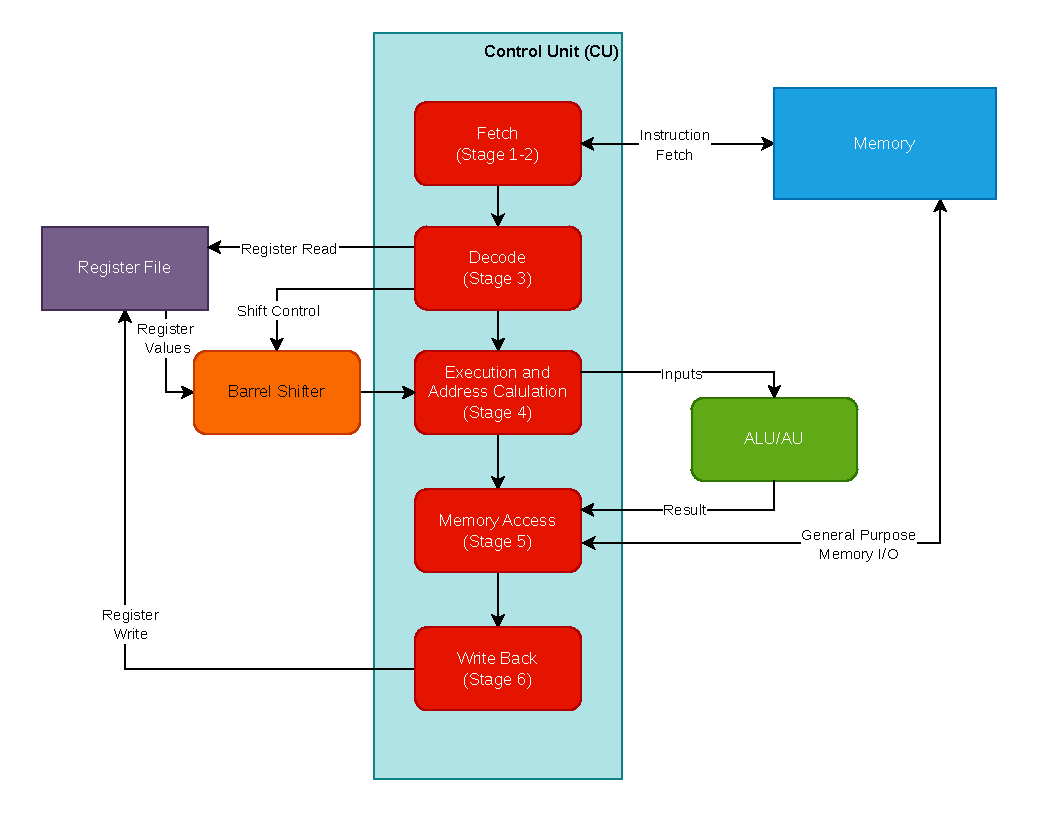
\includegraphics[width=\textwidth]{diagrams/cpu-block-diagram.pdf}
	\caption{SIRC-1 CPU Execution Phase Architecture}
	\label{fig:cpu-block-diagram}
\end{figure}

%TODO: Update the diagram so that the memory component is obviously separate to the other components that live together in the chip

\subsection{Control Unit (CU)}

The Control Unit sits at the heart of the SIRC-1 CPU, coordinating all other functional units throughout the
instruction execution phases. It decodes instructions and generates control signals that orchestrate data movement and
operations across the CPU.

Key responsibilities include:
\begin{itemize}
	\item Instruction fetch and decode
	\item Execution phase coordination
	\item Control signal generation for all functional units
	\item Condition code evaluation for conditional execution
\end{itemize}

\subsection{Arithmetic Logic Unit (ALU)}

The ALU performs all arithmetic and logical operations on register values. It supports the following operations:

\begin{itemize}
	\item \textbf{Arithmetic:} Addition, Subtraction (with and without carry)
	\item \textbf{Logical:} AND, OR, XOR
	\item \textbf{Comparison:} Test and compare operations
	\item \textbf{Status Flag Generation:} Carry, Overflow, Negative, Zero
\end{itemize}

The ALU operates exclusively on data from the Register File (after optional shifting) and outputs results either back
to the Register File or to memory via the data bus.

\subsection{Addressing Unit (AU)}

The Addressing Unit calculates memory addresses and manages address-related operations. It is responsible for:

\begin{itemize}
	\item Computing effective addresses from base + displacement
	\item Handling pre-decrement and post-increment addressing modes
	\item Updating address register pairs (l, a, s, p) for LDEA, jump, and branch instructions
	\item Presenting calculated addresses to the address bus
\end{itemize}

The AU works in parallel with the ALU during the execution stage, allowing address calculation to occur simultaneously
with ALU operations.

\subsection{Register File}

The Register File contains all CPU registers organized into three categories:

\begin{itemize}
	\item \textbf{General Purpose Registers:} \reg{r1}--\reg{r7}
	\item \textbf{Address Register Pairs:} \reg{l} (link), \reg{a} (address), \reg{s} (stack), \reg{p} (program counter)
	\item \textbf{Status Register:} \reg{sr}
\end{itemize}

The Register File provides multi-port access, allowing the ALU, AU, and Control Unit to read and write registers as
needed during each execution phase. All registers are 16 bits wide, though address register pairs can be combined to
form 24-bit addresses.

\subsection{Barrel Shifters}

A barrel shifter sits between the Register File and the CU, enabling efficient bit manipulation operations.

The barrel shifters support logical shift left (\mnemonic{LSL}), logical shift right (\mnemonic{LSR}), arithmetic shift
left (\mnemonic{ASL}), arithmetic shift right (\mnemonic{ASR}), rotate left (\mnemonic{RTL}), and rotate right
(\mnemonic{RTR}). Shift amounts can be specified as immediate values or dynamically from register contents.

The shift is applied to the first source operand when fetching the source registers for an instruction. Shifts cannot
be applied to the result or any other source operand.

\section{Design Characteristics}

\subsection{Combinatorial Logic Implementation}

The SIRC-1 uses pure combinatorial logic with no microcode engine. Each execution phase is implemented as combinatorial
circuits that process data in a single clock cycle. This approach:

\begin{itemize}
	\item Simplifies the hardware design
	\item Provides a deterministic, fixed execution sequence
	\item Eliminates the complexity of microcode sequencing
	\item Makes the CPU behavior fully predictable and easy to reason about
\end{itemize}

\subsection{Fixed Execution Sequence}

Ordinary instructions execute in exactly 6 phases, regardless of instruction type or operands, and complete in 6 clock
cycles when no bus wait states are required. Delayed bus acknowledgement can hold a phase and add wait cycles.
Coprocessor calls are the exception: the processing-unit instruction takes six cycles and the coprocessor dispatch that
follows takes a further six; DMA commands additionally hold instruction fetch until the transfer completes. This design
choice simplifies software timing and eliminates the need for branch prediction or complex multi-stage control logic
found in variable-time architectures.

\subsection{Parallel Functional Units}

The ALU and AU operate in parallel during phase 3 (Execute and Address Calculation), allowing address calculation to
proceed simultaneously with arithmetic operations. This parallelism enables efficient execution of memory reference
instructions without additional clock cycles.

\section{External Interface}

The SIRC-1 CPU exposes its bus, interrupt, and reset signals as physical pins; the chip package, the pin-by-pin descriptions, and the bus timing diagrams are given in Appendix~\ref{appendix:external-interface}. One architectural fact the rest of this chapter relies on: on \texttt{RSTI} assertion the CPU aborts the current instruction or bus wait and restarts at phase 0, as described in the six-stage execution phases above.

\chapter{Register Model}
\label{ch:registers}

\section{Overview}

The SIRC-1 CPU provides sixteen 16-bit registers, classified into three categories:

\begin{itemize}
	\item General-purpose registers (\reg{r1}--\reg{r7})
	\item Address register pairs (\reg{l}, \reg{a}, \reg{s}, \reg{p})
	\item Status register (\reg{sr})
\end{itemize}

All programmer-visible registers are 16 bits wide. Address registers can be used in pairs to form 24-bit addresses for
memory operations.

Only \reg{sr} (cleared to zero) and the \reg{p} pair (loaded from the reset vector) have defined values after reset;
all other registers are architecturally undefined. See Chapter~\ref{ch:exceptions}.

\section{Programming Model}

Figure~\ref{fig:user-programming-model} shows every register a protected-mode program can access directly: the seven
general-purpose registers, the low (unprivileged) word of each of the four address register pairs, and the
unprivileged low byte of \reg{sr}. \reg{sr}'s high byte is shown shaded because it reads as zero and cannot be
written directly in protected mode; see Section~\ref{sec:privilege-restrictions} below.

\begin{figure}[H]
	\centering
	\begin{bytefield}[bitwidth=1.1em]{16}
		\bitheader{0,15} \\
		\bitbox{16}{\reg{r1}} \\
		\bitbox{16}{\reg{r2}} \\
		\bitbox{16}{\reg{r3}} \\
		\bitbox{16}{\reg{r4}} \\
		\bitbox{16}{\reg{r5}} \\
		\bitbox{16}{\reg{r6}} \\
		\bitbox{16}{\reg{r7}} \\
		\bitbox{16}{\reg{ll} (link, low word)} \\
		\bitbox{16}{\reg{al} (address, low word)} \\
		\bitbox{16}{\reg{sl} (stack, low word)} \\
		\bitbox{16}{\reg{pl} (program counter, low word)} \\
		\bitbox{8}{\color{sircgray}\reg{sr} high byte (hidden)} & \bitbox{8}{\reg{sr} low byte}
	\end{bytefield}
	\caption{User Programming Model}
	\label{fig:user-programming-model}
\end{figure}

Figure~\ref{fig:supervisor-programming-model} shows what supervisor mode adds on top of the user programming model:
the high (privileged) word of each address register pair, and \reg{sr}'s high byte, both hidden from a protected-mode
program.

\begin{figure}[H]
	\centering
	\begin{bytefield}[bitwidth=1.1em]{16}
		\bitheader{0,15} \\
		\bitbox{16}{\reg{lh} (link, high word)} \\
		\bitbox{16}{\reg{ah} (address, high word)} \\
		\bitbox{16}{\reg{sh} (stack, high word)} \\
		\bitbox{16}{\reg{ph} (program counter, high word)} \\
		\bitbox{8}{\reg{sr} high byte} & \bitbox{8}{\color{sircgray}\reg{sr} low byte (same as user model)}
	\end{bytefield}
	\caption{Supervisor Programming Model Supplement}
	\label{fig:supervisor-programming-model}
\end{figure}

Table~\ref{tab:register-encoding} below lists every register's encoding and states exactly which ones are
privileged; see Section~\ref{sec:privilege-restrictions} for the full read/write privilege rules.

\section{General-Purpose Registers}

\subsection{Register Set}

The SIRC-1 provides seven general-purpose registers:

\begin{center}
	\begin{tabular}{cl}
		\toprule
		\textbf{Register} & \textbf{Description}       \\
		\midrule
		\reg{r1}          & General-purpose register 1 \\
		\reg{r2}          & General-purpose register 2 \\
		\reg{r3}          & General-purpose register 3 \\
		\reg{r4}          & General-purpose register 4 \\
		\reg{r5}          & General-purpose register 5 \\
		\reg{r6}          & General-purpose register 6 \\
		\reg{r7}          & General-purpose register 7 \\
		\bottomrule
	\end{tabular}
\end{center}

The programmer may use these registers for any purpose. They hold 16-bit values and may be used as source or
destination operands for all ALU instructions.

\subsection{Usage Conventions}

The CPU does not enforce any register-usage convention among \reg{r1}--\reg{r7}; all seven registers are equally
general purpose. Calling conventions and register-preservation rules are outside the scope of this document and are
addressed in the SIRC-1 ABI and Toolchain documentation.

\section{Address Register Pairs}

\subsection{Overview}

The SIRC-1 provides four address register pairs, each consisting of a high and low 16-bit register. When used together,
these pairs form 24-bit addresses by combining the low 8 bits of the high register with the full 16 bits of the low
register.

\begin{figure}[H]
	\centering
	\begin{bytefield}[bitwidth=0.8em]{32}
		\bitheader{0-31} \\
		\bitbox{8}{\color{sircgray}Unused} &
		\bitbox{8}{High Register} &
		\bitbox{16}{Low Register} \\
		\bitbox{8}{\color{sircgray}\tiny bits 31--24} &
		\bitbox{8}{\tiny bits 23--16} &
		\bitbox{16}{\tiny bits 15--0}
	\end{bytefield}
	\caption{Address Register Pair Formation}
	\label{fig:addr-pair}
\end{figure}

The high 8 bits (bits 31--24) of the high register are not used for addressing but remain available for storage,
enabling techniques such as tagged pointers.

The exact address composition and stored-address layout are specified in Chapter~\ref{ch:data-representation}.

Although each address register pair has a specific name and a suggested usage by convention, \mnemonic{STOR} and
\mnemonic{LOAD} instructions treat all four pairs identically, and any pair may be used for indirect addressing.

Loading a value directly into the \reg{p} pair performs a jump.

The link register pair updates automatically when \mnemonic{LDEL}, \mnemonic{LJSR}, or \mnemonic{BRSR} executes. The
program counter pair increments after every instruction.

\subsection{Link Register (l)}

\begin{center}
	\begin{tabular}{ll}
		\toprule
		\textbf{Component} & \textbf{Register}     \\
		\midrule
		High Register      & \reg{lh} (privileged) \\
		Low Register       & \reg{ll}              \\
		\bottomrule
	\end{tabular}
\end{center}

The link register pair stores return addresses for subroutine calls. When a subroutine is called using \mnemonic{LDEL},
\mnemonic{LJSR}, or \mnemonic{BRSR}, the return address is automatically saved to this register pair.

\textbf{Typical Use:}
\begin{itemize}
	\item Storing return addresses from subroutine calls
	\item Alternate storage for general memory addressing
\end{itemize}

\subsection{Address Register (a)}

\begin{center}
	\begin{tabular}{ll}
		\toprule
		\textbf{Component} & \textbf{Register}     \\
		\midrule
		High Register      & \reg{ah} (privileged) \\
		Low Register       & \reg{al}              \\
		\bottomrule
	\end{tabular}
\end{center}

This general-purpose address register pair is used for pointer operations and memory access.

\textbf{Typical Use:}
\begin{itemize}
	\item Base pointer for data structures
	\item Array indexing
	\item General memory addressing
\end{itemize}

\subsection{Stack Pointer (s)}

\begin{center}
	\begin{tabular}{ll}
		\toprule
		\textbf{Component} & \textbf{Register}     \\
		\midrule
		High Register      & \reg{sh} (privileged) \\
		Low Register       & \reg{sl}              \\
		\bottomrule
	\end{tabular}
\end{center}

The stack pointer register pair points to the current top of the stack. Pre-decrement and post-increment addressing
modes are particularly useful with this register.

\textbf{Typical Use:}
\begin{itemize}
	\item Stack operations (push/pop)
	\item Local variable allocation
	\item Function parameter passing
\end{itemize}

\subsection{Program Counter (p)}

\begin{center}
	\begin{tabular}{ll}
		\toprule
		\textbf{Component} & \textbf{Register}     \\
		\midrule
		High Register      & \reg{ph} (privileged) \\
		Low Register       & \reg{pl}              \\
		\bottomrule
	\end{tabular}
\end{center}

The program counter register pair points to the instruction currently being fetched. It is not modified during either
fetch phase; the low word \reg{pl} advances by 2 during the Decode and Register Fetch phase, and \reg{ph} is never
incremented, so a wrap stays inside the segment.

\textbf{Typical Use:}
\begin{itemize}
	\item Automatically updated during normal execution
	\item Modified by branch and jump instructions
	\item Used for position-independent code
\end{itemize}

\section{Status Register}

The status register (\reg{sr}) is a special 16-bit register that contains CPU status flags and control bits. It is
divided into two bytes:

\begin{itemize}
	\item \textbf{Low Byte (bits 7--0):} Condition flags, readable in both modes and updated as a side effect of ALU and
	      shift instructions in both modes; direct writes to \reg{sr} are privileged
	\item \textbf{High Byte (bits 15--8):} Control and privileged state
\end{itemize}

In protected mode, reads of \reg{sr} are redacted to the low byte (high byte reads as zero), and direct writes to
\reg{sr} raise a privilege violation fault. In supervisor mode, a direct write to \reg{sr} is permitted, except that it
cannot change the Exception Active (EA) bit.

The status register is discussed in detail in Chapter~\ref{ch:status-register}.

\section{Privilege Restrictions}
\label{sec:privilege-restrictions}

\subsection{High Address Register Restrictions}

The high component of each address register pair (\reg{lh}, \reg{ah}, \reg{sh}, \reg{ph}) is privileged:

\begin{itemize}
	\item In \textbf{supervisor mode}: Reading and writing are both allowed.
	\item In \textbf{protected mode}:
	      \begin{itemize}
		      \item Reading is allowed.
		      \item Direct writes trigger a privilege exception.
		      \item Address-register-pair write-back is allowed only when the high word would remain unchanged; otherwise it triggers a
		            privilege exception.
	      \end{itemize}
\end{itemize}

This restriction provides a form of memory segmentation and protection. User programs running in protected mode cannot
modify the segment portion of addresses, preventing them from accessing memory outside their designated segment.
Instructions such as \mnemonic{LDEA}, \mnemonic{LDEL}, \mnemonic{BRAN}, \mnemonic{BRSR}, \mnemonic{LJMP},
\mnemonic{LJSR}, and \mnemonic{RETS} remain usable in protected mode when they stay within the current segment. If
their address-register-pair write-back would alter a high word, the CPU raises a privilege violation fault.

The status register differs slightly from the high address registers:
\begin{itemize}
	\item High address registers (\reg{lh}, \reg{ah}, \reg{sh}, \reg{ph}) remain readable in protected mode, but direct writes
	      trigger a privilege violation fault.
	\item The status register's privileged byte is hidden on reads in protected mode, and direct writes in protected mode cannot
	      modify it.
\end{itemize}

\section{Register Addressing}

Registers are addressed using 4-bit register identifiers in instruction encoding:

\begin{table}[H]
	\centering
	\begin{tabular}{clc}
		\toprule
		\textbf{ID}  & \textbf{Register} & \textbf{Privileged}                                 \\
		\midrule
		\texttt{0x0} & \reg{r1}          & No                                                  \\
		\texttt{0x1} & \reg{r2}          & No                                                  \\
		\texttt{0x2} & \reg{r3}          & No                                                  \\
		\texttt{0x3} & \reg{r4}          & No                                                  \\
		\texttt{0x4} & \reg{r5}          & No                                                  \\
		\texttt{0x5} & \reg{r6}          & No                                                  \\
		\texttt{0x6} & \reg{r7}          & No                                                  \\
		\texttt{0x7} & \reg{sr}          & Reads: high byte redacted. Writes: fully privileged \\
		\texttt{0x8} & \reg{lh}          & Yes                                                 \\
		\texttt{0x9} & \reg{ll}          & No                                                  \\
		\texttt{0xA} & \reg{ah}          & Yes                                                 \\
		\texttt{0xB} & \reg{al}          & No                                                  \\
		\texttt{0xC} & \reg{sh}          & Yes                                                 \\
		\texttt{0xD} & \reg{sl}          & No                                                  \\
		\texttt{0xE} & \reg{ph}          & Yes                                                 \\
		\texttt{0xF} & \reg{pl}          & No                                                  \\
		\bottomrule
	\end{tabular}
	\caption{Register Encoding}
	\label{tab:register-encoding}
\end{table}

Because writes to \reg{sr} are fully privileged, any instruction whose destination field encodes \texttt{0x7} is
privileged in protected mode, even when the operation would only alter the unprivileged low byte of \reg{sr}. This
register-index assignment is deliberate: \reg{sr} does not occupy field \texttt{0x0} (unlike an earlier revision of
this encoding), so an all-zero instruction word decodes as \mnemonic{ADDI[N]} \reg{r1}, \texttt{\#0} -- a genuine,
always-unprivileged no-op. This is what lets erased or uninitialized memory (which reads back as all-zero words) be
executed safely instead of faulting; see the \mnemonic{NOOP} entry in Chapter~\ref{ch:meta-instructions}.

\section{Usage Examples}

\begin{example}
	\begin{lstlisting}
; Load immediate value into r1
LOAD r1, #100

; Add 2 to the value stored in r1 and store the result into r2
LOAD r2, r1
ADDI r2, #2

; Add r1 and r2, store in r3
ADDR r3, r1, r2
	\end{lstlisting}
	\caption{Basic Register Operations}
\end{example}

\begin{example}
	\begin{lstlisting}
; Load value from memory at address in 'a' register pair
LOAD r1, (a)

; Store r1 to memory at address (a + 8)
STOR (#8, a), r1

; Push r1 onto stack (pre-decrement)
STOR -(s), r1

; Pop stack into r2 (post-increment)
LOAD r2, (s)+

	\end{lstlisting}
	\caption{Address Register Usage}
\end{example}

\begin{example}
	\begin{lstlisting}
; Call subroutine at address in 'a' register
; Return address saved to 'l' register automatically
LJSR a

; ...subroutine code...

; Return from subroutine
; Copies 'l' register to 'p' register
RETS
	\end{lstlisting}
	\caption{Subroutine Call}
\end{example}

\input{chapters/04-status-register}
\chapter{Exception and Interrupt Handling}
\label{ch:exceptions}

\section{Overview}

An exception is an event that causes the program flow to be diverted to an address stored in a predefined vector.

Some are directly caused by an instruction, some are a side effect of an instruction and some are asynchronously caused
by external hardware.

They are managed by the exception coprocessor, which will take control of the processor when there is a pending
exception.

\section{Exception Types}

\subsection{Abort Exceptions (Faults)}

When an Abort Exception occurs, the instruction causing the exception does not have any effect (it is cancelled after
decode stage). The program address stored in the link register is the address of the faulting instruction so it can be
retried (RETE will return to the same instruction again) This is important for things like privilege violation because
you don't want the illegal instruction to modify any state. These are also referred to as faults. The vectors for abort
exceptions are in the 0x1-0xF range.

\begin{itemize}
	\item \textbf{Bus Fault:} Raised when an external device raised an error via the bus error CPU pin.

	      This could happen, for example, if a unmapped address is presented by the CPU and another chip detects this and raises
	      an error. It could also be used to implement virtual memory as the instruction is aborted and program counter is not
	      incremented, so the address can be re-calculated and the operation retried.

	\item \textbf{Alignment Fault:} Raised when fetching instructions if the program counter contains an odd word address

	      This is to simplify fetching as the second word of an instruction is always at pl | 0x1 and ensures that we never have
	      to worry about instructions overflowing segments (e.g. if the first word is at 0xFFFF and the second word at 0x0000)
	      which is a weird edge case that might complicate fetching.

	\item \textbf{Segment Overflow Fault:} Raised with some instructions if the computed address would go outside the current segment.

	      E.g. if you are accessing data in the stack segment, and then compute an address that overflows, it is probably a stack
	      overflow. There might be situations where you want address calculations to wrap around so it is only raised if the
	      \texttt{TrapOnAddressOverflow} SR bit is set. It is also raised if the program counter overflows, you can tell the
	      difference by reading which phase the fault was raised from the fault metadata register

	\item \textbf{Invalid Opcode Fault:} Raised when a co-processor call is done for a non-existant co-processor
	      or if the co-processor opcode is invalid.

	      Can be used for forward compatibility. For example, if the next iteration of the CPU included a floating point
	      co-processor programs written for that co-processor would trap on the older iteration of the CPU and the floating point
	      operation could be emulated in software. Note: There is no invalid opcode detection for CPU instructions outside of
	      co-processor calls This is just to keep things simple. There is a risk of people using undocumented instructions and
	      those programs breaking in future iterations of the CPU but it is expected that the core of the CPU will remain stable
	      and future ISA improvements will be done via co-processors.

	\item \textbf{Privilege Violation Fault:} Raised when not in supervisor mode and a privileged operation is performed:
	      \begin{enumerate}
		      \item Writing to the high word of any address registers
		      \item Writing to the high byte of the SR register
		      \item Triggering exception below 0x80
	      \end{enumerate}

	\item \textbf{Instruction Trace Fault:} Raised after every instruction when the \texttt{TraceMode} SR bit is set

	      Used for debugging

	\item \textbf{Level Five Hardware Exception Conflict:} Raised when a level five hardware exception is raised
	      when one is already being handled

	      We don't use a stack for handling exceptions, so there is nowhere to store the return address past level five. We could
	      just ignore any level five HW exceptions while it is masked, but that could indicate a hardware misconfiguration, so it
	      is handy so that hardware bugs for things that should not be interrupted are picked up. Level 5 interrupts should be
	      treated like NMIs.

	\item \textbf{Double Fault:} Raised when a fault occurs while another fault is already being handled

	      When the CPU is already handling a fault (priority 7) and another fault occurs, there is no additional banked link
	      register available to store the return address. In this situation, a double fault is raised instead. The double fault
	      mechanism overwrites the fault link register (register 6) with the new return address, meaning there is no way to
	      return to the original program unless the original fault handler stored the return address elsewhere.

	      The fault metadata register (register 7) is also overwritten with information about the double fault. The metadata
	      includes a double fault flag and stores both the current fault type (which will be \texttt{DoubleFault}) and the
	      original fault type that triggered the double fault.

	      The CPU jumps to vector 0x06 (the double fault vector). This is typically used as a last-chance handler to dump
	      registers and reset the CPU. A robust operating system might save the original return addresses in every fault handler
	      to enable recovery from double faults.

	      If a fault occurs while handling a double fault, it will trigger another double fault, continuously overwriting the
	      link registers in an infinite loop. The double fault vector should therefore be implemented with extreme care to avoid
	      any operations that could trigger additional faults.

\end{itemize}

\subsection{Hardware Exceptions (Interrupts)}

A hardware exception occurs when interrupt pins are signalled by external hardware. These are also referred to as
"interrupts". When a hardware exception occurs the current instruction is completed, and control is transferred to
different vectors based on the interrupt "priority". The vectors for hardware exceptions are in the 0x10-0x50 range.

\subsection{User Exceptions (Traps)}

A user exception occurs when the program executes an EXCP instruction that signals the exception coprocessor that it
should trigger an exception. They are usually used by programs running in protected mode to switch to supervisor mode
in a controlled way. They are also referred to as "traps". The vectors for user exceptions are in the 0x60-0xFF range.

\section{Exception Registers}

The SIRC-1 exception coprocessor maintains several special-purpose registers for exception handling.

\subsection{Link Registers}

The exception unit uses banked link registers to store the processor state when an exception occurs. There are eight
link registers in total, indexed 0-7:

\begin{itemize}
	\item Register 0: Software exceptions (traps)
	\item Registers 1-5: Hardware exceptions (interrupts), one for each priority level
	\item Register 6: Faults (abort exceptions)
	\item Register 7: Fault metadata (stores bus address and execution phase information, see section
	      \ref{sec:fault-metadata-register-format} for the format)
\end{itemize}

Each link register stores two pieces of information:

\begin{itemize}
	\item \textbf{Return Address:} The 32-bit address to return to when the exception handler completes
	\item \textbf{Return Status Register:} The 16-bit status register value at the time of the exception
\end{itemize}

When an exception occurs, the appropriate link register (determined by the exception priority level) is populated with
the current program counter and status register values. For abort exceptions (faults), the return address is the
address of the faulting instruction so it can be retried. For regular exceptions (hardware and software exceptions),
the return address is the address after the current instruction.

\subsubsection{Link Register Preservation}

\textbf{Important:} Link registers can be overwritten when fault occurs during fault handling.
A overwrites both the fault link register (register 6)
and the fault metadata register (register 7). This means the original return address is lost.

A valid way of handling this is just to declare the CPU state as invalid, do some last chance error handling (e.g.
dumping the registers) and reset.

For robust fault handling that can recover from double faults, fault handlers should save the link register contents
early in the handler:

\begin{lstlisting}
:fault_handler
    ; Immediately save link register to memory before doing anything
    ; that might trigger another fault
    ETFR #6                   ; Save level 6 exception registers to a and r7
    STOR (s)-, r7
    STOR (s)-, ah
    STOR (s)-, al
    ETFR #7                   ; Save level 7 (metadata) exception registers to a and r7
    STOR (s)-, r7
    STOR (s)-, ah
    STOR (s)-, al

    ; Now safe to perform operations that might fault
    ; ...

    ; Restore and return
    LOAD al, +(s),
    LOAD ah, +(s)
    LOAD r7, +(s)
    ETTR #7                  ; Restore level 6 exception registers from a and r7
    LOAD al, +(s)
    LOAD ah, +(s)
    LOAD r7, +(s)
    ETTR #6                  ; Restore level 7 (metadata) exception registers from a and r7

	; Now save to use RETE
	RETE

\end{lstlisting}

However, if the stack pointer is invalid in this case, the double fault will still cause the CPU state to be corrupted.
You could provide an even more robust implementation by storing/loading from hardcoded memory addresses that are known
to always be valid.

\subsubsection{Fault Metadata Register Format}
\label{sec:fault-metadata-register-format}

The fault metadata register (register 7) stores additional information about faults beyond just the return address. The
return\_status\_register field is used to encode fault-specific metadata in the following format:

\begin{itemize}
	\item \textbf{Bits 0-2:} Execution phase when the fault occurred (3 bits)
	      \begin{itemize}
		      \item 0x0: Instruction fetch
		      \item 0x3: Effective address calculation
		      \item Other values indicate other pipeline phases
	      \end{itemize}
	\item \textbf{Bit 3:} Double fault flag (1 bit) - set to 1 if this is a double fault
	\item \textbf{Bits 4-7:} Current fault type (4 bits) - the type of fault that occurred
	\item \textbf{Bits 8-11:} Original fault type (4 bits) - only meaningful for double faults, indicates the fault type
	      that was being handled when the double fault occurred
	\item \textbf{Bits 12-15:} Unused (reserved for future use)
\end{itemize}

The return\_address field of register 7 stores the bus address that was being accessed when the fault occurred (for
faults that involve memory access). For faults like invalid opcode that occur before bus access, this field will be
zero.

Exception handlers can use the \texttt{ETFR} instruction to read the fault metadata register and decode this
information to determine how to handle the fault appropriately.

\subsection{Cause Register}

The cause register is a 16-bit internal register used to communicate between different CPU units and coordinate
exception handling. It has the following structure:

\begin{itemize}
	\item \textbf{Bits 15-12 (First Nibble):} Coprocessor ID (0x1 for exception unit, 0x0 for processing unit)
	\item \textbf{Bits 11-8 (Second Nibble):} Coprocessor opcode (the operation to execute)
	\item \textbf{Bits 7-0 (Third and Fourth Nibbles):} Vector or parameter value
\end{itemize}

The cause register is automatically populated by the exception unit when a pending exception needs to be serviced. The
priority of exceptions is determined by examining the first nibble of the vector ID, calculated as 7 minus the value of
the first nibble (e.g., 0x00 is priority 7, 0x40 is priority 3, 0x60 and above are all priority 1).

\subsection{Hardware Interrupt Enable Bits}

The status register contains 4 individual enable bits (bits 9-12 in the privileged byte) that control whether each
maskable hardware interrupt line can trigger an exception:

\begin{itemize}
	\item Bit 9 (E1): Hardware Interrupt Line 1 (Level 1, lowest maskable priority)
	\item Bit 10 (E2): Hardware Interrupt Line 2 (Level 2)
	\item Bit 11 (E3): Hardware Interrupt Line 3 (Level 3)
	\item Bit 12 (E4): Hardware Interrupt Line 4 (Level 4, highest maskable priority)
\end{itemize}

\textbf{Note:} Hardware Interrupt Line 5 (Level 5) is a Non-Maskable Interrupt (NMI) and cannot be disabled.
It will always trigger an exception when asserted, regardless of the enable bit settings. Bit 13 is used for the
Exception Active flag instead.

When an interrupt line is disabled (bit = 0), interrupts on that line are completely ignored and not queued. When
enabled (bit = 1), the interrupt can trigger an exception if its priority is higher than the currently executing
exception level.

\textbf{Hierarchical Exception Handling:}

Exceptions in SIRC-1 are strictly hierarchical. A hardware interrupt can only interrupt the current execution if its
priority level (exception level) is \textit{higher} than the currently active exception level. This prevents:

\begin{itemize}
	\item An interrupt handler from being interrupted by its own interrupt (same level)
	\item Lower priority interrupts from interrupting higher priority handlers
	\item Software exceptions from running during any hardware interrupt (would corrupt link register 0)
\end{itemize}

The exception unit maintains a \texttt{current\_exception\_level} field that tracks the active exception level (0-7).
When not handling any exception, this is 0. When handling an exception at level N, only exceptions at level > N can
interrupt.

\section{Exception Processing}

\subsection{Exception Priority}

Exceptions are prioritized as follows (highest to lowest):

\begin{enumerate}
	\item Priority 7: Faults (abort exceptions)
	\item Priority 6: Level 5 hardware exceptions (NMI-like)
	\item Priority 5: Level 4 hardware exceptions
	\item Priority 4: Level 3 hardware exceptions
	\item Priority 3: Level 2 hardware exceptions
	\item Priority 2: Level 1 hardware exceptions
	\item Priority 1: Software exceptions (traps)
\end{enumerate}

\subsection{Exception Handling Flow}

When an exception occurs, the following steps are executed:

\begin{enumerate}
	\item For hardware exceptions, the exception unit checks if the interrupt line is enabled in the status register. If
	      disabled, the interrupt is ignored and not queued.

	\item The exception unit checks if the exception priority level is higher than the current active exception level. If not,
	      the exception is deferred until the current handler completes.

	\item For level 5 hardware exceptions being raised when one is already being handled (both have exception level 6), a Level
	      Five Hardware Exception Conflict fault is raised instead.

	\item The current program counter, status register, and current exception level are stored in the appropriate link register
	      based on the exception priority level.

	\item The Protected Mode bit in the status register is cleared, switching the CPU to supervisor mode.

	\item The current exception level is updated to the level of the exception being serviced.

	\item The vector address is computed by multiplying the vector ID by 2 (since vectors are 32-bit addresses stored as two
	      16-bit words).

	\item The program counter is set to the vector address, transferring control to the exception handler.
\end{enumerate}

\textbf{Returning from Exceptions:}

The RETE (Return from Exception) instruction restores the saved state from the link register:

\begin{enumerate}
	\item The return address is loaded from the link register into the program counter
	\item The saved status register value is restored (including interrupt enable bits)
	\item The saved exception level is restored to current\_exception\_level
	\item Execution resumes at the return address
\end{enumerate}

After RETE, any pending interrupts that are now eligible to run (higher priority than the restored exception level and
enabled) will be serviced before the next instruction executes.

\subsection{Vector Table}

The exception vectors are stored starting at address 0x0. Each vector is a 32-bit address stored as two consecutive
16-bit words. The vector table layout is:

\begin{itemize}
	\item \textbf{0x00:} Reset vector
	\item \textbf{0x01:} Bus fault
	\item \textbf{0x02:} Alignment fault
	\item \textbf{0x03:} Segment overflow fault
	\item \textbf{0x04:} Invalid opcode fault
	\item \textbf{0x05:} Privilege violation fault
	\item \textbf{0x06:} Double fault
	\item \textbf{0x07:} Reserved
	\item \textbf{0x08-0x0F:} Reserved for future privileged exceptions
	\item \textbf{0x10:} Level 5 hardware exception vector
	\item \textbf{0x20:} Level 4 hardware exception vector
	\item \textbf{0x30:} Level 3 hardware exception vector
	\item \textbf{0x40:} Level 2 hardware exception vector
	\item \textbf{0x50:} Level 1 hardware exception vector
	\item \textbf{0x60-0xFF:} User exception vectors (128 user-accessible trap vectors)
\end{itemize}

\section{Return from Exception}

To return from an exception handler, the \texttt{RETE} (Return from Exception) instruction is used. This instruction
performs the following operations:

\begin{enumerate}
	\item Reads the link register corresponding to the current interrupt mask level (minus 1, since the mask is set to the
	      exception level)
	\item Restores the status register from the link register (including the interrupt mask and protected mode bit)
	\item Restores the program counter from the link register
	\item Execution continues from the restored address
\end{enumerate}

For abort exceptions (faults), \texttt{RETE} returns to the faulting instruction, allowing it to be retried. For
regular exceptions, \texttt{RETE} returns to the instruction following the one that was executing when the exception
occurred.

\subsection{Accessing Link Registers}

The exception coprocessor provides instructions to transfer data to and from the link registers:

\begin{itemize}
	\item \textbf{ETFR (Exception Transfer From Register):} Copies the return address and/or status register from a link register to the address register and/or R7
	\item \textbf{ETTR (Exception Transfer To Register):} Copies the address register and/or R7 to a link register's return address and/or status register
\end{itemize}

These instructions allow exception handlers to examine or modify the saved processor state before returning, enabling
features like system calls, context switching, and debuggers.

\section{Exception Coprocessor Instructions}

The exception coprocessor (coprocessor ID 0x1) provides several specialized instructions for exception handling and
system control.

\begin{table}[H]
	\centering
	\begin{tabular}{llll}
		\toprule
		\textbf{Instruction} & \textbf{Opcode} & \textbf{Privilege} & \textbf{Purpose} \\
		\midrule
		\mnemonic{EXCP}      & 0x1             & User                & Trigger a software exception (trap) \\
		\mnemonic{WAIT}      & 0x9             & Supervisor          & Enter wait state until an exception occurs \\
		\mnemonic{RETE}      & 0xA             & Supervisor          & Return from an exception handler \\
		\mnemonic{RSET}      & 0xB             & Supervisor          & Reset CPU state and jump to reset vector \\
		\mnemonic{ETFR}      & 0xC             & Supervisor          & Copy saved exception state from a link register \\
		\mnemonic{ETTR}      & 0xD             & Supervisor          & Write CPU register state back to a link register \\
		\bottomrule
	\end{tabular}
	\caption{Exception Coprocessor Instruction Summary}
	\label{tab:exception-coprocessor-summary}
\end{table}

For full syntax, operation details, and worked examples, see Chapter~\ref{ch:meta-instructions}.

\subsection{Internal Instructions}

The following opcodes are used internally by the exception unit and are not directly accessible via user instructions:

\begin{itemize}
	\item \textbf{Fault (0xE):} Automatically invoked when a fault condition is detected
	\item \textbf{HardwareException (0xF):} Automatically invoked when a hardware interrupt is signaled
	\item \textbf{None (0x0):} No operation, used when no exception is pending
\end{itemize}

These internal operations follow the standard exception handling flow described in the Exception Processing section.


% Part II: Instruction Set Architecture
\part{Instruction Set Architecture}
\input{chapters/06-instruction-formats}
\input{chapters/07-addressing-modes}
\input{chapters/08-shift-operations}
\input{chapters/09-condition-codes}

% Part III: SIRCIS Instruction Reference
\part{SIRCIS Instruction Reference}
\input{chapters/10-instruction-summary}
\input{chapters/11-alu-instructions}
\input{chapters/12-memory-instructions}
\input{chapters/13-control-flow}
\input{chapters/14-coprocessor-instructions}
\input{chapters/15-meta-instructions}

% Back Matter
\appendix
\input{chapters/appendix-a-opcode-map}
\input{chapters/appendix-b-timing}
\input{chapters/appendix-c-undocumented}
\chapter{Example Programs}
\label{ch:example-programs}

This appendix contains sample programs that demonstrate several features of the CPU.

\section{Byte Sieve}

This program computes primes below 1000 using the Sieve of Eratosthenes, storing one byte
per candidate number in a memory-mapped array rather than in a register or the stack. It is
a compact illustration of addressing-register setup (\reg{ah}/\reg{al} and \reg{sh}/\reg{sl})
and of using \mnemonic{STOR} and \mnemonic{LOAD} with an indexed effective address to walk an
array. The two nested loops starting at labels \texttt{:2} and \texttt{:3} (lines 35--50) are
the core of the sieve: the outer loop advances the candidate, and the inner loop marks its
multiples as composite.

% These example programs are too long to fit a non-breaking [H] float, so they use
% \lstinputlisting's own (page-breaking) caption directly rather than the "example" float
% used elsewhere in the manual, while still stepping the shared example counter and adding a
% matching "List of Examples" entry so they appear there too, consistently numbered.
\refstepcounter{example}
\label{ex:byte-sieve}
\addcontentsline{loe}{example}{\protect\numberline{\theexample}Byte sieve}
\lstinputlisting[caption={Example~\theexample: Byte sieve}]{../../examples/byte-sieve/byte-sieve.sasm}

\section{Faults}

This pair of programs exercises every fault type the CPU can raise and the vector table that
routes them to handlers. \texttt{faults.sasm} deliberately triggers, in sequence, a bus fault,
an alignment fault, two segment-overflow faults (one from an effective-address calculation,
one from program-counter overflow), an instruction-trace fault, a bus-protection fault, an
invalid-opcode fault (which itself triggers a nested double fault), a privilege violation, and
a level-five interrupt. Each handler, defined from line 144 onward, increments a distinct
register so a reader can confirm which faults fired and in what order. The segment-overflow
handler (lines 167--204) is worth particular attention: it reads exception metadata with
\mnemonic{ETFR} to distinguish an instruction-fetch overflow from an effective-address
overflow before deciding how to fix up the return address.

\refstepcounter{example}
\label{ex:faults}
\addcontentsline{loe}{example}{\protect\numberline{\theexample}Fault handling}
\lstinputlisting[caption={Example~\theexample: Fault handling}]{../../examples/faults/faults.sasm}

\texttt{faults-high.sasm} is a second, separately assembled segment that the program-counter
overflow test in Example~\ref{ex:faults} jumps into; it exists only to let that fault trigger
without the CPU executing the vector table sitting at address 0x0000 in the main segment. It
jumps back into \texttt{faults.sasm} through the trampoline at 0xFFF0.

\refstepcounter{example}
\label{ex:faults-high}
\addcontentsline{loe}{example}{\protect\numberline{\theexample}High-address fault handling}
\lstinputlisting[caption={Example~\theexample: High-address fault handling}]{../../examples/faults/faults-high.sasm}

\section{Hardware Exception}

This example shows a device-driven interrupt handled through the serial device: the program
prints a help message, waits on \mnemonic{WAIT} for a hardware exception, and exits once the
handler reports that the expected character has arrived in \reg{r7}. The exception handler
itself is installed at vector 0x0080 and defined from line 137 onward; it saves the link
register, calls \texttt{read\_pending\_byte} and \texttt{write\_pending\_byte} in turn, and
restores the link register before returning with \mnemonic{RETE}. Those two subroutines show
the poll-and-acknowledge pattern used to drain and refill the serial device's receive and
send buffers one byte at a time.

\refstepcounter{example}
\label{ex:hardware-exception}
\addcontentsline{loe}{example}{\protect\numberline{\theexample}Hardware exception}
\lstinputlisting[caption={Example~\theexample: Hardware exception}]{../../examples/hardware-exception/hardware-exception.sasm}

The data segment below supplies the two zero-terminated, word-per-character messages
(\texttt{help\_message} and \texttt{exit\_message}) that Example~\ref{ex:hardware-exception}
prints at startup and on exit.

\refstepcounter{example}
\label{ex:hardware-exception-data}
\addcontentsline{loe}{example}{\protect\numberline{\theexample}Hardware exception data}
\lstinputlisting[caption={Example~\theexample: Hardware exception data}]{../../examples/hardware-exception/data.sasm}

\section{Software Exception}

This short program demonstrates a software-raised exception with \mnemonic{EXCP} and confirms
that nesting is blocked while a handler is running. It sets \reg{r1} to 1, raises exception
0x40, and expects \reg{r1} to hold 0xFF once the handler at line 26 has run. That handler
itself raises a second exception, 0x41, from inside the handler; because the handler at vector
0x0500 (line 37) sets \reg{r1} to 0xBB only if it runs, the final value of \reg{r1} shows
whether the nested exception was correctly ignored.

\refstepcounter{example}
\label{ex:software-exception}
\addcontentsline{loe}{example}{\protect\numberline{\theexample}Software exception}
\lstinputlisting[caption={Example~\theexample: Software exception}]{../../examples/software-exception/software-exception.sasm}

\section{Store Load}

This program is a self-checking test of indexed and immediate-offset memory access, followed
by an exhaustive exercise of every \mnemonic{LJMP}/\mnemonic{LJSR} addressing form. The store
and load block (lines 8--19) round-trips values through memory using an immediate offset and a
register offset from an address-register pair. The remainder of the listing chains together
register-offset, immediate-offset, and plain register forms of \mnemonic{LJMP} and
\mnemonic{LJSR}; every path not on the intended route lands on an \texttt{LJMP s}/\texttt{LJSR
s} instruction commented \texttt{FAIL!}, so a working implementation reaches the \texttt{:pass}
label at the end while a faulty one jumps into the "forbidden zone" and fails at \texttt{:fail}.

\refstepcounter{example}
\label{ex:store-load}
\addcontentsline{loe}{example}{\protect\numberline{\theexample}Store/load}
\lstinputlisting[caption={Example~\theexample: Store/load}]{../../examples/store-load/store-load.sasm}


\backmatter
% Index would go here if we add one later

\end{document}
